
% federated-learning.tex

\documentclass[dvipdfmx,notheorems,t]{beamer}

\usepackage{docmute}

% settings.tex

\AtBeginDvi{\special{pdf:tounicode 90ms-RKSJ-UCS2}}

\AtBeginSection[]{\frame[t]{\frametitle{目次}
	\tableofcontents[currentsection,sectionstyle=show/hide,hideallsubsections]}}

\AtBeginSubsection[]{\frame[t]{\frametitle{目次}
	\tableofcontents[currentsection,sectionstyle=show/hide,
	currentsubsection,subsectionstyle=show/shaded/hide]}}

\usefonttheme{professionalfonts}
\usetheme{Madrid}

\setbeamercovered{transparent=30} 
\setbeamertemplate{navigation symbols}{}
\setbeamertemplate{frametitle}[default][left]
\setbeamertemplate{frametitle continuation}{}
\setbeamertemplate{enumerate items}[square]
\setbeamertemplate{caption}[numbered]
\setbeamertemplate{bibliography item}{\insertbiblabel}

\let\oldframe\frame
\renewcommand\frame[1][t,allowdisplaybreaks,allowframebreaks]{\oldframe[#1]}

\usepackage{bxdpx-beamer}
\usepackage{pxjahyper}
\usepackage{minijs}

\usepackage{amsmath}
\usepackage{amssymb}
\usepackage{amsthm}
\usepackage{bm}

\DeclareMathOperator*{\argmax}{arg\,max}
\DeclareMathOperator*{\argmin}{arg\,min}
\DeclareMathOperator{\Tr}{Tr}
\DeclareMathOperator{\KL}{KL}
\DeclareMathOperator{\diag}{diag}

\usepackage[T1]{fontenc}
\usepackage[utf8]{inputenc}

\setbeamertemplate{theorems}[numbered]
\theoremstyle{definition}
\newtheorem{theorem}{定理}
\newtheorem{definition}{定義}
\newtheorem{proposition}{命題}
\newtheorem{lemma}{補題}
\newtheorem{corollary}{系}
\newtheorem{conjecture}{予想}
\newtheorem*{remark}{Remark}
\renewcommand{\proofname}{}

\renewcommand{\figurename}{図}
\renewcommand{\tablename}{表}

\renewcommand{\kanjifamilydefault}{\gtdefault}

\usepackage{url}



\usepackage{animate}

\title[論文輪講: Federated Learning]{論文輪講 \\ Towards Federated Learning at Scale: System Design}
\author{杉浦 圭祐}
\institute[松谷研究室]{慶應義塾大学理工学部情報工学科 松谷研究室}
\date{\today}

\begin{document}

\frame{\titlepage}

\section{}

\begin{frame}[t,allowdisplaybreaks,allowframebreaks]{目次}
\tableofcontents
\end{frame}

\section{Federated Learningの概要}

\begin{frame}{Federated Learningとは}

\begin{itemize}
	\item Federated Learningとは
	\begin{itemize}
		\item \alert{分散機械学習}の新手法 \\
		$\Rightarrow$ 複数のデバイス間に分散したデータを利用し、共通のモデルを学習
		\newline
		\item 既存の分散機械学習の手法とは異なり、プライバシー等の問題を解決 \\
		$\Leftarrow$ 学習は各デバイス上で行われ、その結果が共通のモデルに反映される
	\end{itemize}
\end{itemize}

\end{frame}

\begin{frame}{Federated Learningとは}

\begin{itemize}
	\item 一般的な機械学習との違い
	\begin{itemize}
		\item 学習に使用する訓練データは、クラウド上には保存されない \\
		$\Rightarrow$ 全てのデータは、各デバイスに残されたままである \\
		$\Rightarrow$ \alert{プライバシー}や、データの所有権の問題に対処できる
		\newline
		
		\item クラウド上では、モデルの学習を行わない \\
		$\Rightarrow$ モデルの学習は、各デバイス上で(\alert{オンデバイス}で)行われる \\
		$\Rightarrow$ 学習時には、自身のデバイス上のデータを用いる
		\newline
		
		\item 各デバイスは、モデルを使用した推論だけでなく、学習も行う \\
		$\Rightarrow$ 学習後、クラウド上にある共通のモデルの、パラメータを更新 \\
		$\Rightarrow$ 各デバイスからクラウドへは、モデルの更新情報のみ送信
		\newline
		
		\item 各デバイスで学習されたモデルを、即座に利用できる \\
		$\Rightarrow$ クラウド上のモデルをベースとして、各デバイス向けにカスタマイズ可能
	\end{itemize}
\end{itemize}

\end{frame}

\begin{frame}{Federated Learningとは}

\begin{itemize}
	\item Federated Learningの大まかな流れ
	\begin{enumerate}
		\item 各デバイスが、クラウド上にある現在のモデルをダウンロードする \label{enum:fl-flow-begin}
		\newline
		\item デバイス上のデータを使って、モデルを学習する
		\newline
		\item 学習が終わったら、モデルのパラメータの変更内容(差分)をまとめる
		\newline
		\item 差分をクラウドに送信し、クラウド上の共通のモデルに反映させる \label{enum:fl-flow-end}
		\newline
		\item (\ref{enum:fl-flow-begin})から(\ref{enum:fl-flow-end})までを、繰り返し行う
	\end{enumerate}
\end{itemize}

\end{frame}

\begin{frame}{Federated Learningとは}

\begin{figure}
	\centering
	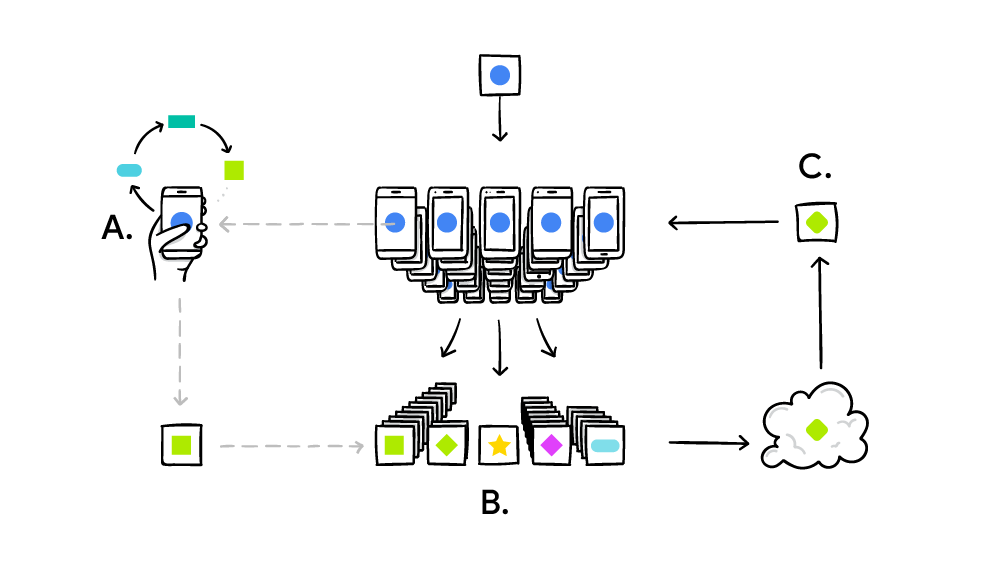
\includegraphics[keepaspectratio, scale=0.3]{federated-learning-flow.png}
	\caption{Federated Learningの流れ~\cite{mcmahan_ramage_2017}}
	\label{fig:federated-learning-flow}
\end{figure}

\end{frame}

\section{イントロダクション}

\begin{frame}{システムの概要}

\begin{itemize}
	\item システムの概要
	\begin{itemize}
		\item モバイル端末(Androidのスマートフォン)を対象としたシステム
		\newline
		\item スケーラブルかつ、実際の製品にもデプロイ可能なレベル \\
		$\Leftarrow$ Gboard(Google Keyboard)というキーボードアプリで実際に使用
		\newline
		\item 実装には、TensorFlowが用いられている \\
		$\Leftarrow$ 深層ニューラルネットの学習も可能である
		\newline
		\item 同期型の訓練アルゴリズム(\alert{Federated Averaging})を採用
		\item セキュリティ向上のための手法(\alert{Secure Aggregation})を利用可能
	\end{itemize}
\end{itemize}

\end{frame}

\begin{frame}{同期型の訓練アルゴリズム}

\begin{itemize}
	\item \alert{同期型}の訓練アルゴリズムが採用された
	\begin{itemize}
		\item 具体的には、\alert{Federated Averaging}というアルゴリズムを使用 \\
		$\Leftarrow$ SGD(Stochastic Gradient Descent)とよく似ている \\
		$\Leftarrow$ SGDを、重み付きの更新によって拡張したような手法
	\end{itemize} \
	
	\item クラウド上のモデルが更新されるまでの流れ
	\begin{enumerate}
		\item 各デバイスから、差分データ(モデルのパラメータの更新情報)を受信
		\newline
		\item \alert{Federated Averaging}を用いて、クラウド上で差分データを一つに集約
		\newline
		\item 集約された差分を、モデルのパラメータに反映(モデルの更新)
		\newline
		\item 更新されたモデルを、各デバイスが取得できるようになる
	\end{enumerate}
\end{itemize}

\end{frame}

\begin{frame}{同期型の訓練アルゴリズム}

\begin{figure}
	\centering
	\includegraphics[keepaspectratio, scale=0.65, clip, trim=1.8cm 13cm 11cm 4cm, page=15]{papers/Towards-Federated-Learning-at-Scale-1902-01046.pdf}
	\label{fig:fl-averaging-algorithm}
\end{figure}

\end{frame}

\begin{frame}{同期型の訓練アルゴリズム}

\begin{itemize}
	\item \alert{同期型}の訓練アルゴリズムが採用された
	\begin{enumerate}
		\item 近年、同期型の訓練アルゴリズムを採用する動きがみられるため \\
		$\Leftarrow$ 同期処理の負担が大きなデータセンタですら、同期型の訓練アルゴリズムを採用する傾向
		\newline
		
		\item プライバシーを強化する手法を適用するため \\
		$\Leftarrow$ Differential PrivacyやSecure Aggregationなどの手法がある \\
		$\Leftarrow$ これらは原則として、同期型のアルゴリズムでないと適用不可能
		\newline
		
		\item サーバ側での処理が単純になるため \\
		$\Leftarrow$ 多数のユーザ(デバイス)からの更新データをまとめて、モデルに適用
	\end{enumerate} \
	
	\begin{itemize}
		\item 但し、同期処理のオーバヘッドを軽減するための対策が必要(後述)
	\end{itemize}
\end{itemize}

\end{frame}

\begin{frame}{セキュリティ向上のための手法}

\begin{itemize}
	\item セキュリティ向上のための手法を利用可能
	\begin{itemize}
		\item 具体的には、\alert{Secure Aggregation}という手法を利用可能 \\
		$\Leftarrow$ 各デバイスから送信される差分データは、外部から隠される
		\newline
		
		\item Federated Learningでは、訓練データは各デバイス上に留まる \\
		$\Leftarrow$ 訓練データには、個人を特定するに足る情報が含まれるかもしれない \\
		$\Leftarrow$ クラウド上にデータを保存しないことで、プライバシーが確保される
		\newline
		
		\item データは送信しない代わりに、データを元に算出した差分データを送信 \\
		$\Leftarrow$ 差分データには、各デバイスを特定するのに十分な情報が、依然として含まれる可能性 \\
		$\Leftarrow$ 差分データをも隠蔽することで、セキュリティを更に向上させられる
	\end{itemize}
\end{itemize}

\end{frame}

\begin{frame}{システムを実装する上での課題}

\begin{itemize}
	\item システムを実装する上での課題が非常に多い
	\begin{enumerate}
		\item デバイスが常に接続されているとは限らない \\
		$\Leftarrow$ デバイス(スマートフォン)の接続状態は不安定になりがち
		\newline
		
		\item デバイスが常に計算可能とは限らない \\
		$\Leftarrow$ 計算が途中で中断させられるかもしれない \\
		$\Leftarrow$ デバイスは世界中に散らばって存在するため、地理的な要因(タイムゾーンなど)を考慮する必要がある
		\newline
		
		\item 複数のデバイスの同期処理を取るのが困難 \\
		$\Leftarrow$ 前述の通り、これらのデバイスは接続状態が不安定で、常に利用できるかどうかも分からない
		\newline
		
		\item デバイスの計算能力とストレージの制限が厳しい \\
		$\Leftarrow$ 深層ニューラルネットの場合はパラメータ数が多く、メモリと計算資源の消費が特に大きい
	\end{enumerate}
\end{itemize}

\end{frame}

\begin{frame}{システムを実装する上での課題}

\begin{itemize}
	\item これらの課題を3つの構成要素で解決
	\begin{itemize}
		\item \alert{通信プロトコル}、\alert{デバイス}、\alert{サーバ}
		\item この3つの動作について、これからみていく
		\newline
		
		\item 論文の著者によれば、このシステムは数百万、あるいは十億台のデバイス上で利用可能だとしている
	\end{itemize}
\end{itemize}

\end{frame}

\begin{frame}{システムを実装する上での注意点}

\begin{itemize}
	\item デバイス上でFederated Learningを無条件に開始してはならない
	\begin{itemize}
		\item デバイスのパフォーマンスを劣化させてはいけない
		\newline
		
		\item Federated Learningが実行されるのは、デバイスが\alert{アイドル状態}で、\alert{充電中}で、かつ\alert{Wi-Fiに接続}されているときのみ \\
		$\Rightarrow$ Federated Learningのために、ユーザがデバイスを使えなくなってしまうのでは、本末転倒 \\
		$\Rightarrow$ 次の図\ref{fig:federated-learning-eligibility}を参照
	\end{itemize}
\end{itemize}

\end{frame}

\begin{frame}{システムを実装する上での注意点}

\begin{figure}
	\centering
	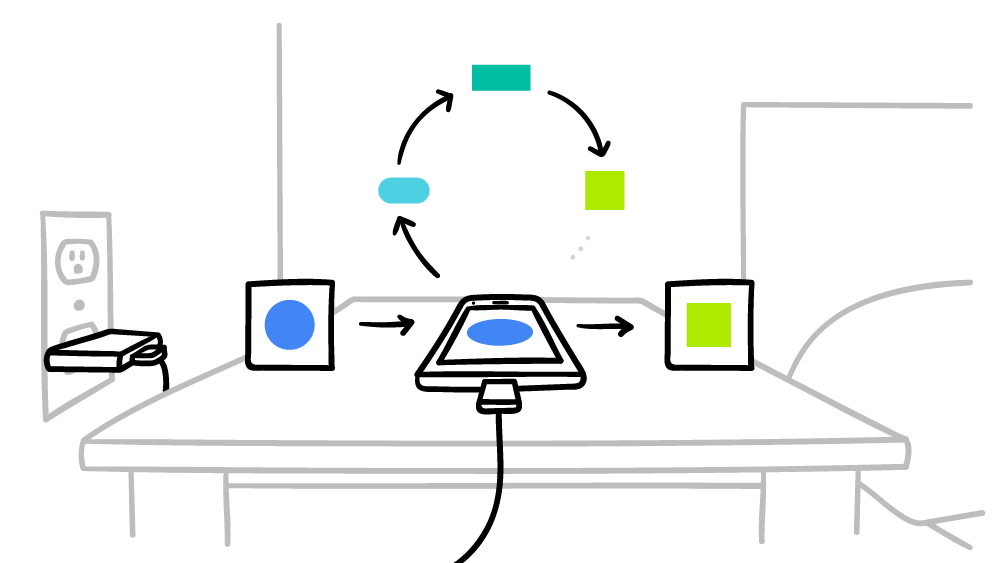
\includegraphics[keepaspectratio, scale=0.3]{federated-learning-eligibility.png}
	\caption{Federated Learningが実行される条件~\cite{mcmahan_ramage_2017}}
	\label{fig:federated-learning-eligibility}
\end{figure}

\end{frame}

\section{通信プロトコル}

\begin{frame}{通信プロトコルの用語整理}

\begin{itemize}
	\item プロトコルの主人公
	\begin{itemize}
		\item デバイス (ここではAndroidのスマートフォン)
		\item \alert{FL Server} (クラウドベースの分散サービス)
	\end{itemize} \
	
	\item \alert{FL Population}
	\begin{itemize}
		\item 学習アルゴリズムで解こうとしている問題
	\end{itemize} \
	
	\item \alert{FL Task}
	\begin{itemize}
		\item 特定の計算タスク \\
		$\Leftarrow$ あるハイパーパラメータが与えられた下での、モデルの訓練 \\
		$\Leftarrow$ デバイス上のローカルなデータを用いた、モデルの評価
		\newline
		\item FL Populationは、複数のFL Taskによって構成される \\
		$\Rightarrow$ FL Taskは、必ず何らかのFL Populationに属する
	\end{itemize}
\end{itemize}

\end{frame}

\begin{frame}{通信プロトコルの用語整理}

\begin{itemize}
	\item \alert{FL Plan}
	\begin{itemize}
		\item FL Taskにおいて、デバイスが行うべき具体的な処理内容
		\item 例えば、モデルの訓練方法や評価手順を表す
		\newline
		
		\item TensorFlowの計算グラフや、タスクの実行方法を格納するデータ構造
	\end{itemize} \
	
	\item \alert{FL Checkpoint}
	\begin{itemize}
		\item クラウド上の現在のモデルのパラメータ
		\item その他の状態 (シリアライズ化されたTensorFlowのセッション)
	\end{itemize} \
	
	\item \alert{Round}
	\begin{itemize}
		\item FL Serverとデバイスとの一連の通信(後述)
		\item \alert{Selection}、\alert{Configuration}、\alert{Reporting}の3段階で構成される
		\item 次の図\ref{fig:fl-protocol}を参照
	\end{itemize}
\end{itemize}

\end{frame}

\begin{frame}{Federated Learningのプロトコル}

\begin{figure}
	\centering
	\includegraphics[keepaspectratio, scale=0.6, clip, trim=2cm 15.5cm 2cm 2.5cm, page=2]{papers/Towards-Federated-Learning-at-Scale-1902-01046.pdf}
	\caption{Federated Learningのプロトコル~\cite{1902.01046}}
	\label{fig:fl-protocol}
\end{figure}

\end{frame}

\begin{frame}{Federated Learningのプロトコル}

\begin{itemize}
	\item Federated Learningのプロトコルの大まかな流れ
	\begin{enumerate}
		\item FL Serverは、ある決められた時間だけ、デバイスからの報告を待機 \label{enum:fl-protocol-begin} \\
		$\Leftarrow$ ある特定のFL Taskが実行可能であることの報告を待つ
		\newline
		\item 多数のデバイスが、指定されたFL Taskを実行可能であることを、FL Serverに伝達
		\newline
		\item FL Serverは、報告してきた数千のデバイスの中から、数百程度のデバイスを選択 \label{enum:fl-protocol-device-selection}
		\newline
		\item 選ばれた数百のデバイスで、FL Taskを実行する \label{enum:fl-protocol-end}
		\newline
		\item (\ref{enum:fl-protocol-begin})から(\ref{enum:fl-protocol-end})までを繰り返す \\
		$\Rightarrow$ この繰り返しの単位をRoundという \\
		$\Rightarrow$ (\ref{enum:fl-protocol-begin})から(\ref{enum:fl-protocol-device-selection})までが\alert{Selection}フェーズ \\
		$\Rightarrow$ (\ref{enum:fl-protocol-end})が\alert{Configuration}と\alert{Reporting}フェーズ
	\end{enumerate}
\end{itemize}

\end{frame}

\begin{frame}{Federated Learningのプロトコル}

\begin{itemize}
	\item Federated LearningのプロトコルのRoundの流れ
	\begin{itemize}
		\item Roundは\alert{Selection}、\alert{Configuration}、\alert{Reporting}の3段階で構成される
		\item Roundの間は、選択されたデバイスはFL Serverとの通信を継続する
		\newline
		
		\item Roundの実行途中で、時間内に応答しないデバイスは\alert{単に無視}される
		\item Federated Protocolのプロトコルは、このようなデバイスの脱落を考慮に入れて設計されている
	\end{itemize}
\end{itemize}

\end{frame}

\begin{frame}{Federated Learningのプロトコル}

\begin{itemize}
	\item Selectionフェーズの流れ
	\begin{enumerate}
		\item FL Taskの実行に適したデバイスは、周期的にFL Serverにアクセス \\
		$\Leftarrow$ \alert{充電中}で、かつ\alert{Wi-Fi}に接続されているデバイス \\
		$\Leftarrow$ 従量課金制のネットワークに接続されたデバイスは、アクセスしない(Federated Learningには参加しない)
		\newline
		
		\item FL Serverにアクセスしたデバイスは、双方向のコネクションを確立 \\
		$\Leftarrow$ Roundの間は、コネクションを維持する必要がある
		\newline
		
		\item FL Serverは、接続してきた数千のデバイスの中から、数百程度のデバイスを選択 \\
		$\Leftarrow$ 1つのRoundには数百程度のデバイスが参加 \\
		$\Leftarrow$ 選択に使用するアルゴリズムは何でもよい(溜池サンプリング)
		\newline
		
		\item 選ばれなかったデバイスに対して、FL Serverは次にアクセスすべき時刻を送信(適当な時間の経過後に、再接続させる)
	\end{enumerate}
\end{itemize}

\end{frame}

\begin{frame}{Federated Learningのプロトコル}

\begin{itemize}
	\item Selectionフェーズで指定可能なパラメータの例
	\begin{itemize}
		\item FL Taskの実行に協力して欲しいデバイスの数(希望)
		\item FL Taskの実行に最低限必要なデバイスの数(閾値)
		\item FL Serverがデバイスからの接続を待つべき時間(タイムアウト)
	\end{itemize} \
	
	\begin{itemize}
		\item 希望通りの数のデバイスが接続してきた時点で、Roundの実行が開始
		\item タイムアウトになるまでは、接続デバイス数が希望通りになるまで待機
		\newline
		\item タイムアウト時に、接続デバイス数が閾値を超えていなければ、Roundは実行されない
	\end{itemize}
\end{itemize}

\end{frame}

\begin{frame}{Federated Learningのプロトコル}

\begin{figure}
	\centering
	\includegraphics[keepaspectratio, scale=0.6, clip, trim=2cm 15.5cm 2cm 2.5cm, page=2]{papers/Towards-Federated-Learning-at-Scale-1902-01046.pdf}
	\caption{Federated Learningのプロトコル(再掲)~\cite{1902.01046}}
\end{figure}

\end{frame}

\begin{frame}{Federated Learningのプロトコル}

\begin{itemize}
	\item Configurationフェーズの流れ
	\begin{enumerate}
		\item 選択されたデバイスに対して、FL Planを送信 \\
		$\Leftarrow$ FL Planは、TensorFlowの計算グラフや、FL Taskの実行方法を格納
		\newline
		
		\item 続いて、選択されたデバイスに対して、FL Checkpointを送信 \\
		$\Leftarrow$ FL Checkpointは、モデルのパラメータや、FL Taskの実行に必要な様々な情報を格納 \\
		$\Leftarrow$ シリアライズ化されたTensorFlowのセッションオブジェクトなど
		\newline
		
		\item デバイスは、FL Serverから渡された情報を元に、FL Taskを実行 \\
		$\Leftarrow$ デバイス上に保存されたデータを用いた、モデルの訓練や評価
	\end{enumerate}
\end{itemize}

\end{frame}

\begin{frame}{Federated Learningのプロトコル}

\begin{itemize}
	\item Reportingフェーズの流れ
	\begin{enumerate}
		\item FL Serverは、デバイスから結果が送信されるのを待機 \\
		$\Leftarrow$ FL Taskがモデルの訓練であれば、差分データ(モデルのパラメータの更新情報)の送信を待機
		\newline
		
		\item FL Serverは、Federated Averagingを使って、差分データを一つに集約 \\
		$\Leftarrow$ 集約された差分を、モデルのパラメータに反映(モデルの更新)
		\newline
		
		\item FL Serverは、タスクを実行し終えたデバイスに対して、次にアクセスすべき時刻を送信 \\
		$\Leftarrow$ 適当な時間の経過後に、デバイスがFL Serverに再接続するように指示
	\end{enumerate} \
	
	\begin{itemize}
		\item 十分な数のデバイスが結果を報告すれば、モデルの更新が実行される
		\item それ以外の場合は、Roundの実行は失敗(無かったことにされる)
	\end{itemize}
\end{itemize}

\end{frame}

\begin{frame}{Federated Learningのプロトコル}

\begin{itemize}
	\item デバイスのFL Serverへの接続頻度の調節
	\begin{itemize}
		\item FL Population(解こうとしている問題)の大きさに応じて、デバイスの接続頻度(一度にFL Serverに接続してくるデバイス数)を調節
		\newline
		
		\item FL Serverは、次に再接続すべき時間を、各デバイスに対して指示する \\
		$\Rightarrow$ この時間をうまく調節することで、デバイスの接続頻度を調節可能
		\newline
		
		\item FL Taskに協力可能(\alert{アクティブ})なデバイスの数は、周期的に変動 \\
		$\Rightarrow$ 充電中で、Wi-Fiに接続されていて、アイドル状態であればアクティブとみなす \\
		$\Rightarrow$ 昼の時間帯は人間が使用するので、アクティブなデバイスが減少 \\
		$\Rightarrow$ それ以外の時間帯(深夜)では、逆にアクティブなデバイスが増加
		\newline
		
		\item これらの周期的な変動も考慮して、再接続までの時間を指定 \\
		$\Rightarrow$ 例えば、昼間の時間帯は、FL Serverにアクセスする頻度を落とす
	\end{itemize}
\end{itemize}

\end{frame}

\begin{frame}{Federated Learningのプロトコル}

\begin{itemize}	
	\item 小さなFL Populationの場合(解こうとしている問題が小さい)
	\begin{itemize}
		\item FL Taskに参加するデバイスの数も少なくて済む
		\newline
		
		\item 十分な数のデバイスが、FL Serverにほとんど同時に接続できるように、接続頻度を上手く調節する \\
		$\Rightarrow$ Selectionフェーズに掛かる時間が短縮 \\
		$\Rightarrow$ 単位時間に実行可能なRoundの数が増加 \\
		$\Rightarrow$ 学習が速やかに進行する
	\end{itemize}
\end{itemize}

\end{frame}

\begin{frame}{Federated Learningのプロトコル}

\begin{itemize}
	\item 大きなFL Populationの場合(解こうとしている問題が大きい)
	\begin{itemize}
		\item 一般的に、FL Taskに協力してくれるデバイスが多数存在する
		\item 但し、一度のRoundに参加するデバイスは、せいぜい数百程度である
		\newline
		
		\item 多数のデバイスが、一度にFL Serverに接続しないようにする \\
		$\Rightarrow$ 一度に多数のデバイスがFL Serverに接続しても、そのうちのごく一部のデバイスが選択され、他の多数のデバイスの接続が無駄になるかもしれない (\alert{Thundering Herd}と呼ばれる問題)
		\newline
		
		\item 各デバイスが、FL Serverにアクセスする時間を、ランダムに決める \\
		$\Rightarrow$ デバイスの接続を時間的に分散させる \\
		$\Rightarrow$ 必要なときに、必要な数のデバイスだけが接続する
	\end{itemize}
\end{itemize}

\end{frame}

\section{デバイス上のソフトウェア}

\begin{frame}{デバイス上のソフトウェア}

\begin{itemize}
	\item デバイス上のソフトウェア
	\begin{itemize}
		\item 今回のシステムは、Androidのスマートフォンが対象
		\item 但し、それ以外のプラットフォームでも実装可能
		\newline
		
		\item アプリケーションプロセス、\alert{FL Runtime}、\alert{Example Store}の3つが連携して動作
		\item この3つは、AndroidのAIDL IPC(Inter Process Communication; プロセス間通信)を使って互いに通信を行う
		\item 次の図\ref{fig:fl-device-arch}を参照
	\end{itemize}
\end{itemize}

\end{frame}

\begin{frame}{デバイス上のソフトウェアのアーキテクチャ}

\begin{figure}
	\centering
	\includegraphics[keepaspectratio, scale=0.8, clip, trim=10.5cm 15.5cm 2cm 5.5cm, page=3]{papers/Towards-Federated-Learning-at-Scale-1902-01046.pdf}
	\caption{デバイス上のソフトウェアのアーキテクチャ~\cite{1902.01046}}
	\label{fig:fl-device-arch}
\end{figure}

\end{frame}

\begin{frame}{デバイス上のソフトウェア}

\begin{itemize}
	\item \alert{Example Store}
	\begin{itemize}
		\item Federated Learningで使用するデータを保存しておくデータベース
		\item クラウド上にあるモデルの学習と、改良に用いられる訓練データ
		\newline
		
		\item 以下のような推奨事項がある
	\end{itemize}
	
	\begin{enumerate}
		\item ストレージを圧迫しないように、データベースの最大容量を、予め決めておく
		\item 各データの保存期間を決めておき、期間を過ぎたデータが自動的に削除されるようにする
		\item マルウェアによる不正アクセスを防止するため、各データを適切に暗号化したうえで保存する
	\end{enumerate}
\end{itemize}

\end{frame}

\begin{frame}{デバイス上のソフトウェア}

\begin{itemize}
	\item \alert{FL Runtime}
	\begin{itemize}
		\item FL Serverとのやり取りを行うソフトウェアのコンポーネント
		\newline
		
		\item FL Taskを実行する際、Example Storeからデータを取得
		\item 取得したデータを用いて、FL Taskで指定された処理(モデルの訓練や評価)を実行する
	\end{itemize}
\end{itemize}

\end{frame}

\begin{frame}{デバイス上のソフトウェア}

\begin{itemize}
	\item デバイス上でのFederated Learningの流れ
	\begin{enumerate}
		\item アプリケーションによるFL Runtimeの設定
		\newline
		\item FL RuntimeがFL Serverにアクセス
		\newline
		\item FL RuntimeがFL Planを実行
		\newline
		\item FL Runtimeが差分データやその他の統計情報をFL Serverに送信
	\end{enumerate}
\end{itemize}

\end{frame}

\begin{frame}{デバイス上のソフトウェア}

\begin{enumerate}
	\item アプリケーションによるFL Runtimeの設定
	\begin{enumerate}
		\item アプリケーションが、FL PopulationとExample Storesを設定する
		\newline
		\item AndroidのJobSchedulerにより、FL Runtimeが周期的に起動される \\
		$\Rightarrow$ 起動されるのは、デバイスが\alert{アイドル状態}で、\alert{充電中}で、\alert{Wi-Fiに接続}されているときのみ \\
		$\Rightarrow$ Federated Learningのためにユーザがデバイスを使えなくなってしまっては本末転倒
		\newline
		\item FL Runtimeは必要ならば、実行途中であっても、強制終了する \\
		$\Rightarrow$ 強制終了するのは、デバイスが上記の3条件を満たさなくなったとき
	\end{enumerate}
	
	\framebreak
	
	\item FL RuntimeがFL Serverにアクセス
	\begin{enumerate}
		\item FL Runtimeがスケジューラによって、アプリケーションとは別のプロセスで起動される
		\newline
		\item FL Runtimeは、FL Taskが実行可能であることを、FL Serverに伝達 \\
		$\Leftarrow$ このFL Taskは、アプリケーションによって設定されたFL Populationに属する
		\newline
		\item FL Serverは、FL Populationに対応したFL Taskがあれば、FL Planを返す
		\newline
		\item FL Taskがない、あるいはデバイスが選択されない場合は、FL Serverは、再接続すべき時間(何分後に再接続すべきか)を返す \\
		$\Rightarrow$ FL Runtimeは終了する \\
		$\Rightarrow$ 指定された時間後に、スケジューラによってFL Runtimeが再度起動される
	\end{enumerate}
	
	\framebreak
	
	\item FL RuntimeがFL Planを実行
	\begin{enumerate}
		\item FL Taskがあり、かつデバイスが選択された場合は、FL PlanがFL Serverから送信される \\
		$\Leftarrow$ FL Planは、FL Taskにおいて、デバイスが行うべき具体的な処理内容が格納されている
		\newline
		\item FL Runtimeは、Example Storeからデバイス上のローカルなデータを取得
		\newline
		\item 取得したデータを使って、FL Planで指示された処理を実行 \\
		$\Rightarrow$ 例えば、データを用いたモデルの訓練 \\
		$\Rightarrow$ 或いは、データを用いたモデルの評価値の計算 \\
		$\Rightarrow$ これは、教師あり学習におけるバリデーションに相当
		\newline
		\item モデルのパラメータの差分や、あるいはモデルの評価結果などを算出
	\end{enumerate}
	
	\framebreak
	
	\item FL Runtimeが差分データやその他の統計情報をFL Serverに送信
	\begin{enumerate}
		\item FL Planの実行後、FL Runtimeが差分データやその他の情報をFL Serverに送信
		\newline
		\item 一時的なリソースを解放して、FL Runtimeが終了 \\
		$\Rightarrow$ 次のFL Runtimeも、スケジューラによって起動される
	\end{enumerate}
\end{enumerate}

\end{frame}

\begin{frame}{デバイス上のソフトウェア}

\begin{itemize}
	\item ソフトウェアの特長
	\begin{enumerate}
		\item 1つのアプリケーションが複数のFL Populationを設定可能 \\
		$\Rightarrow$ 1つのアプリケーションが、複数のモデルに対するタスクを行える \\
		$\Rightarrow$ 但し、デバイスに負荷が掛からないよう、同時に複数のFL Planが実行されることはない
		\newline
		
		\item Federated Learningには匿名で参加する \\
		$\Rightarrow$ 但し、ユーザの情報をFL Serverに送信せずに、正規のユーザであることを確認する必要 \\
		$\Rightarrow$ モデルの学習に影響を与えようとする、不正なデバイスを防止するため
	\end{enumerate}
	
	\begin{itemize}
		\item AndroidのSafetyNet Attestation APIにより実装
		\item 正規のデバイスやアプリケーションのみがFederated Learningに参加する
		\item 悪意のあるデータを学習データとして利用し、学習結果を恣意的に操作する\alert{Data Poisoning}も防止
	\end{itemize}
\end{itemize}

\end{frame}

\section{サーバ上のソフトウェア}

\begin{frame}{サーバ上のソフトウェア}

\begin{itemize}
	\item サーバ上のソフトウェア
	\begin{itemize}
		\item デバイス数や通信データ量は、学習しようとしている問題によって全く異なる
		\newline
		
		\item FL Serverと通信する可能性のあるデバイス数は、FL Populationに応じて様々に変化し得る
		\item \alert{数百台}程度の小規模なものから、\alert{数億台}程度の大規模な問題を扱わなくてはならない
		\item 各Roundに参加するデバイスの台数も、\alert{数十}から\alert{数千}程度になり得る
		\newline
		
		\item 学習されるモデルのサイズ(パラメータ数)や、モデルの差分データのサイズも様々
		\item 各Roundにおいて、FL Serverとデバイス間でやり取りされるデータ量も、\alert{数KB}から\alert{数十MB}の範囲を取り得る
		\newline
		
		\item 時間帯によってアクティブなデバイス数が変動するので、トラフィック量も変動
	\end{itemize}
\end{itemize}

\end{frame}

\begin{frame}{サーバ上のソフトウェア}

\begin{itemize}
	\item サーバ上のソフトウェア
	\begin{itemize}
		\item サーバ上で動作するソフトウェアは、\alert{アクターモデル}に則って実装されている
		\item アクターモデルは、並列計算モデルの一種である
		\newline
		
		\item ソフトウェアの各コンポーネントは、全て\alert{Actor}として扱う
		\item Actor間の通信手段は、(到着順の保証されない)\alert{メッセージパッシング}のみである
		\newline
		
		\item 各Actorは、到着したメッセージを順番に処理してゆく(内部状態が変化する)
		\item メッセージを受信すると、内部状態の変更、他のActorへのメッセージの送信、新たなActorの生成などを行う
	\end{itemize}
\end{itemize}

\end{frame}

\begin{frame}{サーバ上のソフトウェア}

\begin{itemize}
	\item サーバ上のソフトウェア
	\begin{itemize}		
		\item 同じ種類のActorを、複数のプロセッサやマシン上で並列に動作させれば、容易にスケールできる
		\item Actorは、同一のプロセッサやプロセス上に共存してもよいし、複数のマシン上に分散させてもよい
		\newline
		
		\item アクターモデルは、\alert{スケーラビリティ}に優れる(スケールアップとスケールダウンが容易) \\
		$\Rightarrow$ デバイス数や通信データ量が大きく変動するため、スケーラビリティは必須の要件
		\newline
		
		\item FL Serverへの負荷に応じて、Actorの数を動的に変更させる
	\end{itemize}
\end{itemize}

\end{frame}

\begin{frame}{サーバ上のソフトウェア}

\begin{itemize}
	\item サーバ上のソフトウェア
	\begin{itemize}
		\item \alert{Coordinator}、\alert{Master Aggregator}、\alert{Aggregator}、\alert{Selector}の4種類のActorが連携して動作
		\item 次の図\ref{fig:fl-server-arch}を参照
		\newline
		
		\item CoordinatorとSelectorは常に存在するActorである \\
		$\Leftrightarrow$ Master AggregatorとAggregatorは、一時的に存在する(必要に応じて作られる)
	\end{itemize}
\end{itemize}

\end{frame}

\begin{frame}{サーバ上のソフトウェアのアーキテクチャ}

\begin{figure}
	\centering
	\includegraphics[keepaspectratio, scale=0.6, clip, trim=2cm 16.5cm 11cm 2.2cm, page=5]{papers/Towards-Federated-Learning-at-Scale-1902-01046.pdf}
	\caption{サーバ上のソフトウェアのアーキテクチャ~\cite{1902.01046}}
	\label{fig:fl-server-arch}
\end{figure}

\end{frame}

\begin{frame}{サーバ上のソフトウェア}

\begin{itemize}
	\item \alert{Coordinator}
	\begin{itemize}
		\item 最上位に位置するActor
		\item Actor全体の同期を取るほか、Roundの進行を担う
		\newline
		
		\item Coordinatorは複数存在し、各Coordinatorが、1つのFL Populationに対応する
		\item 分散ロック機構によって、各FL Populationに対し、Coordinatorが1つだけ存在することが保証される \\
		$\Leftarrow$ 各Coordinatorが、管理対象のFL Populationを登録するときに、分散ロックを使用
	\end{itemize}
\end{itemize}

\end{frame}

\begin{frame}{サーバ上のソフトウェア}

\begin{itemize}
	\item \alert{Coordinator}と\alert{Master Aggregator}の関係
	\begin{itemize}
		\item Coordinatorは、各FL Task(のRound)に対して1つのMaster Aggregatorを生成 \\
		$\Leftarrow$ FL Taskは、必ず1つのFL Populationに属する \\
		$\Leftarrow$ どのFL Taskが実行されるかは、スケジューリングされている
	\end{itemize} \
	
	\item \alert{Master Aggregator}
	\begin{itemize}
		\item FL Taskの各Roundを管理するActor
		\item スケーラビリティを確保するために、必要に応じた数の\alert{Aggregator}を生成 \\
		$\Leftarrow$ モデルのサイズや、Roundに参加するデバイスの台数に応じて決定
	\end{itemize}
\end{itemize}

\end{frame}

\begin{frame}{サーバ上のソフトウェア}

\begin{itemize}
	\item \alert{Coordinator}と\alert{Selector}の関係
	\begin{itemize}
		\item Coordinatorは、何台のデバイスが各Selectorに接続されているのかを取得 \\
		$\Rightarrow$ 各Selectorに対して、(Roundに参加する)デバイスを何台選択すればよいか指示
		\newline
		
		\item 各SelectorはCoordinatorから、各FL Populationに対して何台のデバイスが必要かを知る \\
		$\Rightarrow$ この情報をもとに、各Selectorに現在接続しているデバイスの中から、何台を選択するか(Roundに参加させるか)を決定する
	\end{itemize}
\end{itemize}

\end{frame}

\begin{frame}{サーバ上のソフトウェア}

\begin{itemize} 
	\item \alert{Selector}
	\begin{itemize}
		\item 各デバイスとの接続を担当するActor
		\newline
		
		\item 複数のSelectorは、地理的に分散して存在できる \\
		$\Rightarrow$ 各Selectorが、その地域のデバイスとの通信を担当する \\
		$\Rightarrow$ Selectorとデバイスとの距離が小さくなる
	\end{itemize}
\end{itemize}

\end{frame}

\begin{frame}{サーバ上のソフトウェア}

\begin{itemize}
	\item \alert{Selector} (続き)
	\begin{itemize}
		\item Coordinatorは、各FL Taskに対して1つのMaster Aggregatorを生成 \\
		$\Rightarrow$ Master Aggregatorは、必要に応じて幾つかのAggregatorを生成 \\
		$\Rightarrow$ その後、SelectorはAggregatorに、選択された(Roundに参加する)デバイスに関する情報を伝達 \\
		$\Rightarrow$ 以後、Aggregatorが、Roundに参加するデバイスを管理
		\newline
		
		\item Coordinatorは、FL Taskをデバイスに効率的に割り振ることが可能 \\
		$\Rightarrow$ 何台のデバイスがアクティブかということは、Coordinatorには関係ない \\
		$\Rightarrow$ FL Serverはアクターモデルを採用することで、スケーラビリティを達成
	\end{itemize}
\end{itemize}

\end{frame}

\begin{frame}{サーバ上のソフトウェア}

\begin{itemize}
	\item FL Taskの実行によって、モデルが更新されるまでの流れ
	\newline
	
	\item Roundの開始
	\begin{enumerate}
		\item Coordinatorが、Roundに応じたMaster Aggregatorを1つ生成
		\newline
		\item Master Aggregatorは、必要に応じた数のAggregatorを生成
	\end{enumerate} \
	
	\item Selectionフェーズ
	\begin{enumerate}
		\item SelectorはCoordinatorに対し、デバイスの接続台数を伝達
		\newline
		\item CoordinatorはSelectorに対し、何台のデバイスを選択すべきか指示
		\newline
		\item Selectorが、Roundに参加させるデバイスを、指定された分だけ選択し、Aggregatorに伝える
	\end{enumerate}
	
	\framebreak
	
	\item Configurationフェーズ
	\begin{enumerate}
		\item Aggregatorは各デバイスに対し、FL Planを配布してタスクの実行を指示
	\end{enumerate} \
	
	\item Reportingフェーズ
	\begin{enumerate}
		\item 各デバイスがタスクを実行し終えたら、Aggregatorに結果(差分データ)をアップロード
		\newline
		\item Aggregator上で結果を集約し、Master Aggregatorに再度アップロード
		\newline
		\item Master Aggregator上で、各Aggregatorから送られてきた結果を集約して、最終的な結果を生成
		\newline
		\item 最終的な結果(差分データ)をモデルに適用する
	\end{enumerate}
\end{itemize}

\end{frame}

\begin{frame}{サーバ上のソフトウェア}

\begin{itemize}
	\item システムの利点
	\begin{itemize}
		\item 各Actorは、内部状態をメモリ上に保持する \\
		$\Rightarrow$ スケーラビリティの確保と、分散ストレージを使わないことによる低レイテンシの実現
		\newline
		
		\item ストレージには、各デバイスから送信された結果は保存しない \\
		$\Rightarrow$ データセンタが攻撃されても、各デバイスに関するデータが漏洩する危険性がない
		\newline
		
		\item プロトコルのパイプライン化を達成 \\
		$\Rightarrow$ 他のRoundがConfigurationやReportingフェーズであるときも、Selectorは次のRoundに参加するデバイスを募集できる \\
		$\Rightarrow$ Selectionフェーズは、以前のRoundとは何の関係もないため \\
		$\Rightarrow$ アクターモデルの採用によって得られる利点
	\end{itemize}
\end{itemize}

\end{frame}

\begin{frame}{サーバ上のソフトウェア}

\begin{itemize}
	\item クラッシュした場合のシステムの動作
	\begin{itemize}
		\item 一部のActorがクラッシュしても、システムは動作を継続できる
		\newline
		
		\item AggregatorやSelectorがクラッシュすると、それらが管理していたデバイスだけが、システムからは消失 \\
		$\Rightarrow$ 他のAggregatorやSelectorと通信するデバイスには、影響がない
		\newline
		
		\item Master Aggregatorがクラッシュすると、管理されていたRoundも消失 \\
		$\Rightarrow$ そのRoundの実行は失敗する \\
		$\Rightarrow$ その後Coordinatorによって、Roundを再度実行するための、Master Aggregatorが生成される
		\newline
		
		\item Coordinatorがクラッシュすると、Selectorがそのことを検知して、再度生成する \\
		$\Rightarrow$ Coordinatorに関する情報は、分散ロックによって管理されている \\
		$\Rightarrow$ 同一のFL Populationに対応するCoordinatorが、複数個生成されることはない
	\end{itemize}
\end{itemize}

\end{frame}

\section{アナリティクス}

\begin{frame}{アナリティクス}

\begin{itemize}
	\item 動作状況の把握のため、次のようなデータを解析した
	\begin{itemize}
		\item Federated Learningが開始したときのデバイスの状態(使用中かどうかなど)
		\item Federated Learningの実行頻度と、継続時間
		\item メモリの使用量
		\item Federated Learningの実行中に発生したエラー
		\item スマートフォンの製品データ、OS、FL Runtimeのバージョン
		\newline
		\item これらの情報には個人を特定できるものは含まれない(本当か?)
	\end{itemize} \
	
	\item サーバ側では次のようなデータを解析した
	\begin{itemize}
		\item Roundに参加したデバイスの台数、リジェクトされたデバイスの台数
		\item Roundの各フェーズ(Selection、Configuration、Reporting)の実行時間
		\item データのアップロードやダウンロード時間、発生したエラー
	\end{itemize}
\end{itemize}

\end{frame}

\begin{frame}{アナリティクス}

\begin{itemize}
	\item 発生した問題の種類
	\begin{itemize}
		\item 適切ではないタイミングでFederated Learningが開始された \\
		$\Leftarrow$ デバイスが充電中でない、アイドル状態でない、Wi-Fiに接続されていないなど \\
		$\Leftarrow$ この類の問題は、ユーザがデバイスを使えなくなるので、発生させてはならない
		\newline
		
		\item Roundに参加できないデバイスの台数が、予想を遥かに上回ることがあった \\
		$\Leftarrow$ ユーザのデバイスに直接影響が及ぶことはない
		\newline
		
		\item ユーザのデバイスの性能に影響を及ぼしているかどうかを、検出するのは困難である
	\end{itemize}
\end{itemize}

\end{frame}

\section{Secure Aggregation}

\begin{frame}{Secure Aggregation}

\begin{itemize}
	\item Secure Aggregationの概要
	\begin{itemize}
		\item Federated Learningのセキュリティを向上させるための手法
		\item 各RoundのReportingフェーズで利用することが可能
		\newline
		
		\item モデルの更新を繰り返して得られる、複数の差分データを集約する \\
		$\Leftarrow$ 各デバイスの、個々の差分データは隠蔽される
		\newline
		
		\item \alert{Honest but Curious}タイプの攻撃者を防止 \\
		$\Leftarrow$ プロトコルに沿った動きをするが、プロトコル上でやり取りされるメッセージから、様々な情報を抜き取ろうとする攻撃者
		\newline
		
		\item \alert{Prepare}、\alert{Commit}、\alert{Finalization}フェーズの3つに分かれる
	\end{itemize}
\end{itemize}

\end{frame}

\begin{frame}{Secure Aggregation}

\begin{itemize}
	\item Prepareフェーズ
	\begin{itemize}
		\item FL Serverとデバイス間での暗号化された通信を確立
	\end{itemize} \
	
	\item Commitフェーズ
	\begin{itemize}
		\item デバイスが、暗号によりマスクされたモデルの差分データを、FL Serverにアップロード
		\item FL Serverは、これらのマスクされた差分データを集約
	\end{itemize} \
	
	\item Finalizationフェーズ
	\begin{itemize}
		\item FL Serverが、デバイスから送信された差分データのマスクを外す \\
		$\Leftarrow$ 各デバイスから、マスクを外すことの許可を受ける必要がある \\
		$\Leftarrow$ 但し、デバイスは許可を与えなくてもよい
	\end{itemize}
\end{itemize}

\end{frame}

\begin{frame}{Secure Aggregation}

\begin{itemize}
	\item スケーラビリティとの兼ね合い
	\begin{itemize}
		\item デバイスの数の二乗に比例して、計算コストが増大 \\
		$\Rightarrow$ 最大でも、数百台程度のデバイスでしか利用できない \\
		$\Rightarrow$ Roundに参加できるデバイスの台数が、制限されてしまう
		\newline
		
		\item Secure Aggregationを、各Aggregator(Actorの一種)で動作させることで対処 \\
		$\Rightarrow$ 各Aggregatorが、それぞれに接続されたデバイスから、モデルの差分データを受信して、一つに集約(ここでSecure Aggregationを使用) \\
		$\Rightarrow$ 各Aggregatorが集約した差分データを、Master Aggregatorが更に一つにまとめ上げる(Secure Aggregationは\alert{未使用})
		\newline
		
		\item Master Aggregatorに計算負荷が集中しにくい \\
		$\Leftarrow$ 複数のAggregatorがSecure Aggregationの処理を分担するため
		\newline
		
		\item Roundに参加するデバイスの台数が制限されない
	\end{itemize}
\end{itemize}

\end{frame}

\section{モデル設計者の作業}

\begin{frame}{モデル設計者の作業}

\begin{itemize}
	\item 中央(クラウド上)にデータを集めて行う、モデルの学習とは大きく異なる
	\begin{itemize}
		\item モデルの設計者は、個々の訓練データを直接見ることができない \\
		$\Leftarrow$ そこで、設計者側で、テストとシミュレーション用の、何らかの仮データを用意する必要がある
		\newline
		
		\item モデルを学習させるためには、一度FL Planを作成して、FL Serverから各デバイスに配布しなければならない \\
		$\Leftarrow$ 設計者が、モデルを直接手元で試すだけでは、十分なテストができない
		\newline
		
		\item 学習はデバイス上で動作する \\
		$\Rightarrow$ デバイス上のリソース消費量や、デバイスとの互換性に配慮する必要がある
	\end{itemize}
\end{itemize}

\end{frame}

\begin{frame}{モデル設計者の作業}

\begin{itemize}
	\item モデル設計者の作業の流れ
	\begin{enumerate}
		\item モデルの設計とシミュレーション
		\item デバイスにタスクを割り振るためのFL Planの作成
		\item バージョン管理、テスト、デプロイ
	\end{enumerate}
\end{itemize}

\begin{figure}
	\centering
	\includegraphics[keepaspectratio, scale=0.6, clip, trim=2cm 21cm 2cm 2.2cm, page=7]{papers/Towards-Federated-Learning-at-Scale-1902-01046.pdf}
	\caption{モデル設計者の作業の流れ~\cite{1902.01046}}
	\label{fig:model-engineer-workflow}
\end{figure}

\end{frame}

\begin{frame}{モデル設計者の作業}

\begin{enumerate}
	\item モデルの設計とシミュレーション
	\begin{itemize}
		\item モデルの定義を行う
		\item モデルの学習と評価を行うためのFL Taskを作成 \\
		$\Leftarrow$ TensorFlowベースの専用のライブラリが用意されている \\
		$\Leftarrow$ 入力のテンソルを、LossやAccuracy値に変換する計算グラフの構築
		\newline
		
		\item FL Taskを、モデルの開発者側が用意したテストデータを使って評価
		\newline
		
		\item スケール可能な、シミュレーションツールを用いて行う \\
		$\Rightarrow$ シミュレーションでは、同一のコードが実行されるほか、デバイスとFL Serverとの通信も完全に再現される \\
		$\Rightarrow$ キーボードアプリであれば、ユーザの入力の代わりに、Wikipediaのコーパスなどをテストデータとする
		\newline
		
		\item シミュレーションで、モデルの事前学習を行うこともできる
		\newline
		
		\item FL Taskには、学習率などのハイパーパラメータも設定
		\item 複数のFL Taskが1つのグループを形成してもよい \\
		$\Rightarrow$ ハイパーパラメータのグリッドサーチなどが例 \\
		$\Rightarrow$ 1つのFL Populationに、複数のFL Taskが含まれていてもよい
	\end{itemize}
	
	\framebreak

	\item デバイスにタスクを割り振るためのFL Planの作成
	\begin{itemize}
		\item 設計者が用意した複数のモデルと、設定内容から、FL Planは自動生成される
		\newline
		
		\item FL Planは2つの部分(FL Server用とデバイス用)に分けられる
		\newline
		
		\item デバイス用の部分には次のような情報が格納される \\
		$\Rightarrow$ TensorFlowの計算グラフ \\
		$\Rightarrow$ Example Store(データベース)から訓練データを選別する基準 \\
		$\Rightarrow$ 訓練データのバッチ化の手順 \\
		$\Rightarrow$ 実行するエポック数 \\
		$\Rightarrow$ モデルのパラメータの保存と読み込みのタイミング
		\newline
		
		\item FL Server用の部分には次のような情報が格納される \\
		$\Rightarrow$ デバイスからの差分データを集約する手順
	\end{itemize}
	
	\framebreak
	
	\item バージョン管理、テスト、デプロイ
	\begin{itemize}
		\item Federated Learningのシステムは、FL Planのバージョン管理、テスト、デプロイを容易にしてくれる \\
		$\Rightarrow$ Federated Learningは、様々なデバイス上で動作する \\
		$\Rightarrow$ あるデバイス上ではメモリ使用量が大き過ぎるかもしれない \\
		$\Rightarrow$ あるいは、(FL Serverとデバイス上で動作する)TensorFlowのバージョンに、ずれ(非互換性)が生じるかもしれない
		\newline
		
		\item TensorFlowのバージョンアップによって、計算グラフに非互換性が生じるかもしれない \\
		$\Rightarrow$ デバイス上では、依然として古いバージョンのFL Runtimeが動作している可能性 \\
		$\Rightarrow$ 同じノードであっても、計算の中身が変わっているかもしれない
		\newline
		
		\item FL Planにはバージョン情報が付加されている \\
		$\Rightarrow$ ある1つのFL Taskから、バージョンの異なる複数のFL Planが生成される \\
		$\Rightarrow$ バージョンが異なっても、(意味的に)同一の計算が実行されるように、適切に計算グラフが書き換えられる \\
		$\Rightarrow$ 同一のテストデータを使って、複数のバージョンのFL Planがテストされる
		\newline
		
		\item FL Planが、FL Serverで受け入れられるための条件 \\
		$\Rightarrow$ FL Planに含まれるコードが、十分に検証されていること \\
		$\Rightarrow$ FL Planはテストデータを含み、そのテストにパスすること \\
		$\Rightarrow$ FL Planが消費するリソース量が、許容範囲内であること \\
		$\Rightarrow$ FL Taskがサポート対象とした、全てのTensorFlowのバージョンで、実際に動作すること
	\end{itemize}
\end{enumerate}

\end{frame}

\section{アプリケーション}

\begin{frame}{アプリケーション}

\begin{itemize}
	\item Federated Learningが適している状況
	\begin{itemize}
		\item 学習データがサーバ上ではなく、個々のデバイス上にある場合 \\
		$\Leftarrow$ 学習データが生成されるのが、サーバ上ではなくデバイス上であるような場合
		\newline
		
		\item 学習データが、プライバシーに関わるような場合
		\item 学習データをサーバに送信するのが好ましくないか、不可能であるような場合
		\newline
		
		\item Federated Learningは、教師あり学習のタスクで主に使用されている \\
		$\Leftarrow$ 教師データは、何らかのユーザの反応であることが多い \\
		$\Leftarrow$ 例えば入力データは、アプリが提示した次の入力単語の候補であり、教師データは、ユーザが実際に入力した単語
	\end{itemize}
\end{itemize}

\end{frame}

\begin{frame}{アプリケーション}

\begin{itemize}
	\item Federated Learningが採用されたアプリケーションの例
	\begin{enumerate}
		\item デバイス上でのアイテムのランク付け \\
		$\Rightarrow$ 例えばスマートフォンの設定画面において、ユーザの検索単語から、設定内容の適切な候補を選び出して提示する機能
		\newline
		
		\item キーボードアプリでのサジェスト機能 \\
		$\Rightarrow$ 入力された文章に応じた、様々なコンテンツのサジェスト機能 \\
		$\Rightarrow$ Gboard (Google Keyboard)というキーボードアプリで実装 \\
		$\Rightarrow$ 次の図\ref{fig:federated-learning-content-suggestion}を参照
		\newline
		
		\item 次の入力単語の予測 \\
		$\Rightarrow$ Gboardで実装された機能で、RNNを用いて次の入力単語を予測
	\end{enumerate}
\end{itemize}

\end{frame}

\begin{frame}{アプリケーション}

\begin{figure}
	\centering
	\animategraphics[loop,controls,width=0.75\linewidth]{20}{./federated-learning-content-suggestion-animation/federated-learning-content-suggestion-}{0}{367}
	\caption{キーボードアプリでのサジェスト機能~\cite{mcmahan_ramage_2017}}
	\label{fig:federated-learning-content-suggestion}
\end{figure}

\end{frame}

\begin{frame}{アプリケーション}

\begin{itemize}
	\item 次の入力単語の予測
	\begin{itemize}
		\item モデルは巨大であり、140万のパラメータを持っていた
		\item パラメータが収束するまでに、約$3,000$回のRoundが実行された
		\item 5日間にわたって、$1.5 \times 10^6$台のデバイス上で、$6 \times 10^8$個の文章が処理された(各Roundの実行時間は2、3分)
		\newline
		
		\item 1番目に表示した単語の選択率が、$13.0\%$から$16.4\%$に上昇
		\item Federated Learningによって得られたモデルは、従来のモデルに比べて性能が良くなった
		\newline
		
		\item サーバ上にデータを集めて、モデルを学習させるのと比べて、パラメータが収束するのに約7倍の時間が掛かった
	\end{itemize}
\end{itemize}

\end{frame}

\section{実際の動作状況}

\begin{frame}{実際の動作状況}

\begin{itemize}
	\item データの不正確さ
	\begin{itemize}
		\item Federated Learningを用いたアプリケーションは、まだ少ない
		\item 動作状況を調べるための統計データは、実際に動作するアプリケーションから得たものである \\
		$\Leftarrow$ 精密な統計データを得るために、特別な環境を整えることはしていない
	\end{itemize} \
	
	\item スケーラビリティ
	\begin{itemize}
		\item Federated Learningのシステムは、デバイスの台数やFL Populationに応じて、適切にスケールする
		\item 現在は、幾つかのアプリケーションと、それらを利用する約1,000万台のデバイスを対象として、Federated Learningのシステムが動作している
	\end{itemize}
\end{itemize}

\end{frame}

\begin{frame}{実際の動作状況}

\begin{itemize}
	\item 接続されたデバイスの台数
	\begin{itemize}
		\item デバイスは適切なときに起動されるほか、接続頻度もFL Populationに応じて調節される \\
		$\Rightarrow$ FL Serverに同時に接続しているデバイスは、1万台程度
		\newline
		
		\item Roundに参加するデバイスの台数は、1日の間で変動する \\
		$\Rightarrow$ 夜間は、アイドル状態かつ充電中であることが多いため、Roundに参加するデバイスが増加する傾向 \\
		$\Rightarrow$ 参加するデバイス数が、最も少ないときと、最も多いときの差は4倍
	\end{itemize}
\end{itemize}

\end{frame}

\begin{frame}{実際の動作状況}

\begin{figure}
	\centering
	\includegraphics[keepaspectratio, scale=1.2, clip, trim=1.9cm 17.2cm 11cm 7.6cm, page=13]{papers/Towards-Federated-Learning-at-Scale-1902-01046.pdf}
	\caption{接続されたデバイスの台数~\cite{1902.01046}}
	\label{fig:connected-devices}
\end{figure}

\end{frame}

\begin{frame}{実際の動作状況}

\begin{figure}
	\centering
	\includegraphics[keepaspectratio, scale=1.2, clip, trim=1.9cm 14.5cm 11cm 9.8cm, page=9]{papers/Towards-Federated-Learning-at-Scale-1902-01046.pdf}
	\caption{1時間あたりのRoundの実行回数~\cite{1902.01046}}
	\label{fig:round-completion-rate}
\end{figure}

\end{frame}

\begin{frame}{実際の動作状況}

\begin{itemize}
	\item Roundに参加したデバイスの台数
	\begin{itemize}
		\item 各Roundには数百台のデバイスが参加すれば、モデルの学習には十分であった \\
		$\Leftarrow$ それ以上の台数のデバイスが参加することの利点がなかった(パラメータの収束時間は改善されない)
		\newline
		
		\item ネットワークの問題、計算時のエラー、計算の中断(ユーザがデバイスを使用したなど)によって、$6\%$から$10\%$のデバイスがRoundから欠落した \\
		$\Rightarrow$ FL Serverは、デバイスのRoundからの欠落を最初から見越して、実際よりも多めのデバイスをRoundに参加させた \\
		$\Rightarrow$ 各RoundのSelectionフェーズにおいて、1.3倍の台数のデバイスを選択した(Federated Averagingのアルゴリズムを参照) \\
		$\Rightarrow$ 昼の方が、夜に比べて欠落するデバイスの割合が高くなった(昼の時間帯は、ユーザによってデバイスが使用され、アイドル状態ではなくなる)
	\end{itemize}
\end{itemize}

\end{frame}

\begin{frame}{実際の動作状況}

\begin{figure}
	\centering
	\includegraphics[keepaspectratio, scale=1.2, clip, trim=10.5cm 21.5cm 2cm 2.2cm, page=13]{papers/Towards-Federated-Learning-at-Scale-1902-01046.pdf}
	\caption{各Roundに参加したデバイスの台数の平均~\cite{1902.01046}}
	\label{fig:devices-per-round}
\end{figure}

\end{frame}

\begin{frame}{実際の動作状況}

\begin{itemize}
	\item Roundの実行時間とデバイスの参加時間
	\begin{itemize}
		\item 殆どのデバイスのRoundへの参加時間は、Roundの実行時間と大体等しい \\
		$\Leftarrow$ FL Serverは、必要な数より少し多めのデバイスを選択する \\
		$\Leftarrow$ そして、必要な数のデバイスから計算結果が返されたら、Roundの実行が終了する \\
		$\Leftarrow$ 従って、殆どのデバイスのRoundへの参加時間は、似たようなものになる
		\newline
		
		\item デバイスのRoundへの参加時間には上限がある \\
		$\Leftarrow$ FL Serverは、結果をなかなか返さない(もたついている)デバイスを単に無視する \\
		$\Leftarrow$ 各RoundのReportingフェーズの時間は、予め決められている
	\end{itemize}
\end{itemize}

\end{frame}

\begin{frame}{実際の動作状況}

\begin{figure}
	\centering
	\includegraphics[keepaspectratio, scale=0.8, clip, trim=10.5cm 13.2cm 2cm 7.8cm, page=13]{papers/Towards-Federated-Learning-at-Scale-1902-01046.pdf}
	\caption{Roundの実行時間とデバイスの参加時間~\cite{1902.01046}}
	\label{fig:round-execution-time}
\end{figure}

\end{frame}

\begin{frame}{実際の動作状況}

\begin{itemize}
	\item ネットワークのトラフィック
	\begin{itemize}
		\item サーバからのダウンロードの方が、サーバへのアップロードよりも多い \\
		$\Leftarrow$ サーバからダウンロードするのは、FL Planと、現在のモデル(いずれも同程度のサイズ) \\
		$\Leftarrow$ サーバへアップロードされるのは、モデルに適用する差分データのみ \\
		$\Leftarrow$ 差分データは、現在のモデルやFL Planに比べて圧縮しやすい
	\end{itemize}
\end{itemize}

\end{frame}

\begin{frame}{実際の動作状況}

\begin{figure}
	\centering
	\includegraphics[keepaspectratio, scale=1.2, clip, trim=10.5cm 6cm 2cm 18.2cm, page=13]{papers/Towards-Federated-Learning-at-Scale-1902-01046.pdf}
	\caption{ネットワークのトラフィック~\cite{1902.01046}}
	\label{fig:server-network-traffic}
\end{figure}

\end{frame}

\begin{frame}{実際の動作状況}

\begin{itemize}
	\item デバイスでの学習状況
	\begin{itemize}
		\item $75\%$のクライアントは、モデルを訓練し終えた後、サーバにアップロードできている
		\newline
		
		\item $22\%$のクライアントでは、モデルの訓練は成功しているが、結果をサーバからリジェクトされている \\
		$\Leftarrow$ 結果のアップロードまでに時間が掛かり、サーバから単に無視されている
		\newline
		
		\item $2\%$のクライアントが、モデルの訓練の途中で強制終了している \\
		$\Leftarrow$ モデルの訓練途中に、ユーザがデバイスを使用し始め、アイドル状態ではなくなったことなどが原因
	\end{itemize}
\end{itemize}

\end{frame}

\begin{frame}{実際の動作状況}

\begin{figure}
	\centering
	\includegraphics[keepaspectratio, scale=1.2, clip, trim=1.9cm 21.2cm 11cm 2.2cm, page=14]{papers/Towards-Federated-Learning-at-Scale-1902-01046.pdf}
	\label{fig:on-device-training-round-sessions}
\end{figure}

\end{frame}

\section{関連研究}

\begin{frame}{関連研究}

\begin{enumerate}
	\item デバイス上のデータを用いたモデルの学習手法
	\begin{itemize}
		\item Pihur et al. (2018)で提案された手法 \\
		$\Rightarrow$ デバイス上で算出した差分データを集約する必要がない \\
		$\Rightarrow$ プライバシーの対策も取られている \\
		$\Rightarrow$ 一般化線形モデルに特化している \newline \newline
		$\Rightarrow$ 非同期型のアルゴリズムであり、デバイスから送信された差分データをサーバに保存する必要がないので、スケーラブルであるとしている \newline \newline
		$\Leftrightarrow$ Federated Learningは同期型であるが、スケーラブルであり、Federated Averagingなどの幾つかの訓練アルゴリズムを使えば、デバイスからの送信データをオンラインに処理でき、サーバ上に保存する必要がない
		\newline
		
		\item Smith et al. (2017)やKamp et al. (2018)で提案された手法 \\
		$\Rightarrow$ Federated Learningと、システムの設計が近い
		
		\framebreak
		
		\item Nishio \& Yonetani (2018)による手法 \\
		$\Rightarrow$ Federated Learningと同様に、同期型のアルゴリズム \\
		$\Rightarrow$ サーバが全てのデバイスにアクセスできるという前提 \\
		$\Rightarrow$ 各デバイスからの差分データは、同期的に受け取る \\
		$\Rightarrow$ Federated Learningでも実装可能
		\newline
		
		\item Federated Learningと似た概念は、以下のような分野で既に提唱されていた \\
		$\Rightarrow$ 自動車同士の通信 [Samarakoon et al., (2018)] \\
		$\Rightarrow$ 医療分野 [Brisimi et al., (2018)]
	\end{itemize}
	
	\framebreak
	
	\item 分散機械学習(Distributed Machine Learning)
	\begin{itemize}
		\item Federated Learningは、デバイスでの学習に特化したシステムである \\
		$\Rightarrow$ データセンタのノードと比べると、通信速度が低く、また信頼性にも劣る
		\newline
		
		\item 分散機械学習とは異なり、あらゆる分散処理の形態に対応しているわけではない \\
		$\Rightarrow$ Federated Learningでは、同期型のプロトコルが採用される \\
		$\Rightarrow$ デバイス上での学習のために、最適化されている
		\newline
		
		\item パラメータサーバはFederated Learningには取り込めない \\
		$\Rightarrow$ パラメータサーバでは、モデルのパラメータに各ワーカーがアクセスし、非同期に更新していく \\
		$\Rightarrow$ デバイス上での学習というより、パラメータ数が$10^9$から$10^{12}$程度の、巨大なモデルを学習させるための、サーバのアーキテクチャに焦点が当てられている \newline \newline
		$\Leftrightarrow$ Federated Learningでは、FL Serverが、Roundに参加するデバイスを選択する手続きがある(パラメータを同期的に更新するため)
	\end{itemize}
	
	\framebreak
	
	\item MapReduce [Dean \& Ghemawat (2008)]
	\begin{itemize}
		\item MapReduceは、機械学習には適さないほか、根本的に異なる \\
		$\Leftarrow$ MapReduceとFederated Learningとの、枠組みは似ている \\
		$\Leftarrow$ FL ServerがReducerで、各デバイスがMapperと対応付けられる
		\newline
		
		\item MapReduceとは前提条件が異なる \\
		$\Rightarrow$ 各デバイスがデータを保持しており、完全に独立して動くActorである \\
		$\Rightarrow$ FL Serverは、適切な(eligible)デバイスを選択するほか、選択されたデバイスの一部から送信されてきた結果を集約する(選択されたデバイスの全てが結果を送信するわけではない) \newline \newline
		$\Rightarrow$ FL Serverは、多くのデバイスが計算を中断すること、デバイスの可用性が極端に変動することを考慮して動作 \newline \newline
		$\Rightarrow$ MapReduceではなく、これらの特殊な環境に合わせたフレームワークを採用すべき
	\end{itemize}
\end{enumerate}

\end{frame}

\section{今後の研究}

\begin{frame}{今後の課題}

\begin{enumerate}
	\item バイアスへの対処
	\begin{itemize}
		\item Federated Learningでは、全てのデバイスが均等に参加し、学習を行うことが前提 \\
		$\Rightarrow$ 学習されるモデルが、バイアスを生む可能性がある
		\newline
		
		\item デバイスは、Wi-Fiに接続され、かつ充電されているときにのみFederated Learningに参加 \\
		$\Rightarrow$ 幾つかの国では、依然としてWi-Fiが普及していない
		\newline
		
		\item 今回のシステムでは、Androidで、メモリを2GB以上搭載した、高性能のデバイスのみ参加 \\
		$\Rightarrow$ これもバイアスを生む原因となる可能性
		\newline
		
		\item 現在のシステムでもバイアスの発生にはある程度対処 \\
		$\Rightarrow$ デバイス上での学習を実行後、アプリケーションに応じた複数の指標を使って、リアルタイムでモデルを評価 \\
		$\Rightarrow$ デバイス上での学習が、モデルの性能に悪影響を与えていないかどうか検出
		\newline
		
		\item 現時点ではバイアスによる影響は生じていない \\
		$\Leftarrow$ 但し、アプリケーションによって、バイアスがどの程度出現するのかは分からない \\
		$\Leftarrow$ 様々なアプリケーション上での評価や、バイアスの影響を軽減するようなアルゴリズムの開発が、今後も必要
	\end{itemize}
	
	\framebreak
	
	\item パラメータの収束速度
	\begin{itemize}
		\item データセンタでの学習と比べて、パラメータの収束が遅い
		\newline
		
		\item 現在のFederated Learningでは、数百のデバイスがRoundに参加して、モデルの学習を実行 \\
		$\Rightarrow$ 実際には沢山のデバイスが、モデルの学習を実行できる状態にある \\
		$\Rightarrow$ アルゴリズムの改良によって、より多くのデバイスがRoundに参加できるようにする
		\newline
		
		\item 各RoundのSelectionフェーズやReportingフェーズの時間は、現在は静的に決定される \\
		$\Rightarrow$ 動的に決定することで、脱落するデバイスの割合や、単位時間あたりのRoundの実行数を改善できる可能性がある \\
		$\Rightarrow$ オンラインの機械学習アルゴリズムによって、パラメータを学習する方法などが考えられる
	\end{itemize}
	
	\framebreak
	
	\item スケジューリングの改善
	\begin{itemize}
		\item デバイス上では、複数のFL Taskを同時に扱うことが可能(1つのFL Taskのみが実行される) \\
		$\Rightarrow$ FL Taskの実行順に関しては特に考慮されていない(キューに入った順番で決定) \\
		$\Rightarrow$ ユーザが、どのアプリケーションを頻繁に使用するかなどを、考慮する余地がある
		\newline
		
		\item FL Taskが、古いデータを使って何度も学習を実行する、あるいは新しいデータを学習に用いないといった処理も考えられる
	\end{itemize}
	
	\framebreak
	
	\item バンド幅
	\begin{itemize}
		\item モデルがRNNであれば、学習データと比較して、パラメータの容量が大きくなるかもしれない \\
		$\Rightarrow$ 単に学習データをサーバにアップロードして、学習を進めた方が、通信量の観点では有利かもしれない \\
		$\Rightarrow$ これはユーザのプライバシーの確保とのトレードオフである
		\newline
		
		\item サーバとデバイス間の通信量を削減するための手法が考えられる \\
		$\Rightarrow$ モデルの圧縮、パラメータの量子化などが挙げられる \\
		$\Rightarrow$ 通信量の削減と、モデルによる推論の効率化を同時に達成可能
	\end{itemize}
	
	\framebreak
	
	\item Federated Learningの一般化(Federated Computation)
	\begin{itemize}
		\item ここで紹介したシステムを応用できるアプリケーションは、まだまだある
		\newline
		
		\item 特定の機械学習の手法に特化したものではない \\
		$\Leftarrow$ FL Plan、モデル、差分データといった抽象的な用語で表現
		\newline
		
		\item Federated Learningの概念を、Federated Computationに拡張できる \\
		$\Rightarrow$ TensorFlowを用いた機械学習に限らず、MapReduceのようなアプリケーションにも適用
		\newline
		
		\item Federated Analyticsを検討している \\
		$\Rightarrow$ デバイス固有の統計情報をクラウドにアップロードすることなく、それらを集約したデータのみをアップロードする \\
		$\Rightarrow$ プライバシーを保護しつつ、開発者は(集約された)デバイスの統計情報を見ることができる
	\end{itemize}
\end{enumerate}

\end{frame}

\begin{frame}{参考文献}

\bibliographystyle{plain}
\bibliography{federated-learning-bibliography}

\end{frame}

\end{document}
